\documentclass[a4paper, 12pt, titlepage]{article}

% Document quality things
\usepackage[utf8]{inputenc}
\usepackage{microtype, xcolor}
\usepackage{csquotes}
\usepackage{url, hyperref}
\hypersetup{colorlinks=true, linkcolor=black, citecolor=black, urlcolor=blue}

% Image-related packages
\usepackage{graphicx}
%\usepackage{float}
\graphicspath{{./gfx/}}
%\usepackage[font=small,skip=5pt]{caption}

% Setting margins
\usepackage[a4paper,bottom=2cm,top=2cm,left=2.5cm,right=2.5cm, includefoot]{geometry}

% Table helper packages
%\usepackage{multirow, multicol}
%\usepackage{makecell}
%\usepackage{array}
%\usepackage{tabularx} % Not needed currently, but has a few nice options
%\usepackage{wrapfig} % Floating figures/tables
\usepackage{booktabs}
\usepackage{longtable}
\usepackage{diagbox}

% Prevents spamming tedious newlines everywhere, also disables auto indentation, etc.
\usepackage[skip=0.75\baselineskip plus 2pt]{parskip}

% Self-explanatory
%\usepackage{titlesec}
%\titleformat{\section}[block]{\normalfont\scshape\Large}{\thesection}{1em}{}
%\titleformat{\subsection}{\normalfont\large}{\thesubsection}{1em}{}

\title{
    {CS 319 - Object Oriented Software Engineering}\\
    {\small Instructor: Eray Tüzün, TA: Muhammad Umair Ahmed \& Elgun Jabrayilzade}\\
    {\vspace{10mm}BilHealth}\\
    {\Large \textbf{Design Report}}\\
    {\small Iteration 2}\\
    {\vspace{10mm}
\includegraphics[width=0.3\linewidth]{bilkentlogo}}
}
\author{
  Mehmet Alper Çetin\\ \texttt{21902324}
  \and
  Vedat Eren Arıcan\\ \texttt{22002643}
  \and
  Uygar Onat Erol\\ \texttt{21901908}
  \and
  Recep Uysal\\ \texttt{21803637}
  \and
  Efe Erkan\\ \texttt{21902248}
}
\date{\today}

% \usepackage{tikz}
% \usetikzlibrary{automata, positioning, arrows}

\usepackage{pdflscape, pdfpages}

\begin{document}
  \maketitle
  \tableofcontents
  \pagebreak

  \section{Introduction}

  Our project is a health center management software, built in the form a web application.
  This report documents the design choices that were made for the implementation of the project.

  Note that all diagrams on this document are in vector format, meaning that you can zoom in without any decrease in quality.

  \subsection{Purpose of the System}

  The project is designed as a web-based application that will ease the health center management in Bilkent.
  The main goal of the project is to provide online attention to the patients
  and to have better communication betweeen doctors, staff and patients.
  Our system includes features that ease the interaction betweeen patients and doctors through cases
  which contain all relevant information for a given medical situation.
  Patients can open cases and request for appointments through that opened cases.
  Also, staff and doctors provide patients with medical services through cases.

  \subsection{Design Goals}

  \subsubsection{Accessibility}

  The system should be accessible by all actors despite individual shortcomings, to achieve its goal.
  We want to design a user interface such that a person who isn't familiar with using
  computers can easily find their way around the website.
  All the buttons and labels in the system should have self-explanatory titles.
  The system should include boundary conditions which prevent the user from taking wrongful actions.

  As a general guideline to practices that make up an accessible user interface,
  the \href{https://developer.mozilla.org/en-US/docs/Web/Accessibility}{Mozilla Developer Network} and
  \href{https://www.w3.org/standards/webdesign/accessibility}{World Wide Web Consortium (W3C)} are useful.

  \subsubsection{Security}

  The system will have a person's health details which are highly privacy sensitive.
  Also, the system will have confidential information of every user such as Bilkent ID,
  email address and password. Therefore, the system should be secure to protect
  all of these personal information from any unauthorized activity.
  No user would want such private data to be accessed by any unauthorized person.

  To secure the app, the implementation should follow an access control schema as such:

  \begin{itemize}
    \item A doctor can access a patient's full profile only while the doctor is assigned to an open case with the patient.
    \item A nurse can access a patient's full profile only while granted permission by the patient or a staff member.
      This access should expire after some amount of time.
    \item A staff member can always access a patient's full profile.
      However, this access is fully tracked, also known as an \textit{audit trail}.
  \end{itemize}

  From research, this schema appears to align with health information security practices around the globe.

  \subsubsection{Performance}

  The system should give the best performance even on computers with old hardware.
  Every user interaction should be processed and displayed in less than 1 second to provide
  a better experience to the user.

  In order to ensure sufficient performance, potential bottleneck points should be addressed.
  One of the most notorious bottlenecks is database access.
  The system should limit round trips to the database as much as possible.
  When data is queried or written, it should be done with transactions that allow all of the process to be completed
  on a single request.

  \subsubsection{Scalability}

  The system aims to support up to 20 thousand users, which means the design should enable concurrency and high throughput.

  \subsubsection{Deployment}

  In order to facilitate the development of the project in a fast paced environment,
  the design takes into consideration concepts such as portability and replicability.
  The sought result is that developers can easily run a local version of the system while
  keeping things simple when the time comes to deploy to production.

  \subsubsection{Testability}

  Almost any respectable web service of today strives to achieve test driven development of some magnitude.
  Our project is no different and the design attempts to make it possible to incorporate unit or integration tests
  for the business logic, by means such as dependency injection.

  \subsubsection{Extensibility and Maintainability}

  The fast paced development environment can quickly turn the project into a nightmare of spaghetti code and architecture.
  To counteract such a possibility, the design aims to keep components maintainable and extensible through proven OOP structs.

  \subsection{Top Two Design Goals}

  For the implementation of the health center management software, two primary design goals were chosen:
  \textbf{Security} and \textbf{Scalability}.

  Due to the fact that the system contains sensitive health information about the users, such as diagnosis and test results,
  the system should be secure to prevent unauthorized access. In addition to this, data should be stored in a secure way
  in order to prevent possible identity thefts. Therefore, \textbf{security} is chosen to be one of the top design goals.

  The health center management system may have up to 20.000 end users, and these users may execute operations on the system concurrently.
  Therefore, in order to prevent any issues, scalability is chosen to be one of the top design goals.

  \section{High-Level Software Architecture}

  \subsection{Subsystem Decomposition}

  Since the project uses React as its front-end interface technology, the subsystems are not divided according to views.
  The front-end client, \texttt{APIClient}, handles all communication with the API exposed by the \textit{controller layer}.
  To elaborate, this client component sends HTTP requests to the back-end endpoints according to the user's interactions with React.

  The service layer is called by the controller layer to execute the business logic and database access required to perform a given action.
  The data layer consists of the domain models, powered by the Entity Framework Core library.

  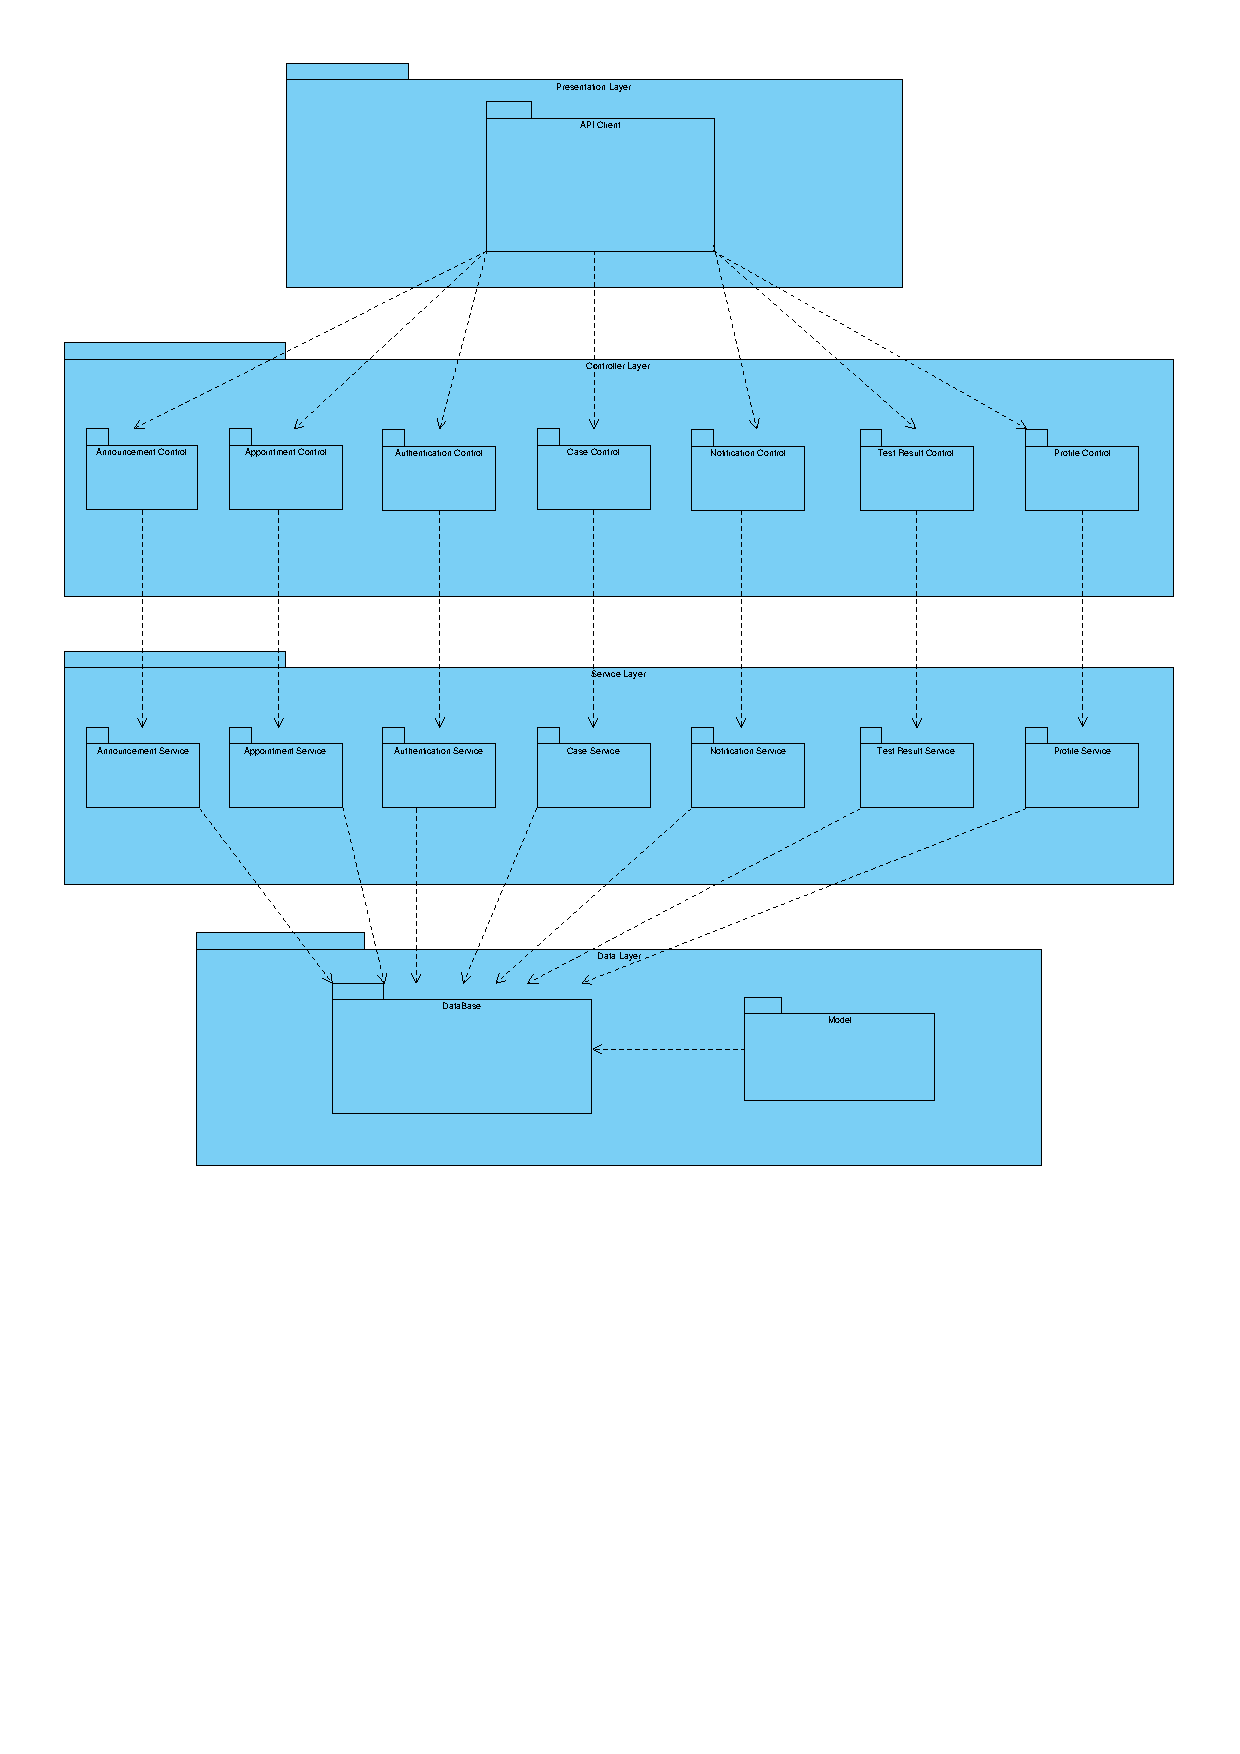
\includegraphics[width=\linewidth]{subsystem}

  \subsection{Hardware-Software Mapping}

  The project does not have any extraordinary hardware requirements.
  As it is a web application, it requires the users to have a device using which they can
  connect to the web server of the application over the internet.
  The main target devices for a supported user experience are desktop computers, laptops, and mobile phones.

  In order to run the project the intended way, the host system's hardware must support stable containerization through Docker.
  It is possible to reconfigure certain entrypoints of the project to support bare-metal execution too, at the cost of
  system replicability and practicality.
  Similar to most other web services, the project is officially supported to run on a Linux environment, which
  may be of consideration when choosing hardware.

  The server on which the system runs should have the following specifications at a minimum:

  \begin{itemize}
    \item A server-grade CPU such as Intel Xeon, with clockrates above 2.0 GHz
    \item 16-32 GB of RAM to support many users and interactions at once
    \item 1-2 TB of storage to support the database and the test result store
  \end{itemize}

  \subsection{Persistent Data Management}

  The project makes use of PostgreSQL as its persistent data storage solution.
  The project does not have specific requirements that directly justify the use of PostgreSQL,
  however, this database system is well rounded enough to save the development process from any potential drawbacks.
  The \texttt{psql} command line tool is easy to use and supports our workflow in implementing database migrations.
  Also, the Docker images for the database are robust and simple,
  which has allowed the project to be supported by a containerized database.

  On top of the actual database, the project uses EF Core as an object relational mapper (ORM),
  which is Microsoft's official library for data persistence.
  We use the recommended \textit{code-first} approach of database management, which means our PostgreSQL tables are
  constructed by EF Core with respect to our entity definitions in C\# code.
  The EF Core toolchain generates migrations, which it also converts to SQL scripts,
  using which a database can be configured to host the project in moments.

  All of the domain models seen on the class diagrams are persisted to the database.

  \subsection{Access Control and Security}

  The project is secured by a typical authentication and authorization flow,
  supported by our identity provider of choice, ASP.NET Core Identity.
  Authentication is conducted over HTTPS with a user's username and password.
  The controller endpoints of the project are exposed to users within specific role types,
  which constitutes our authorization process.
  The authentication is persisted on the user's device in the form of browser cookies, enabling user session capability.

  The project is mostly exclusive to authenticated users, meaning that there are not many substantial actions a guest user can take.
  Moreover, since users are divided across roughly 5 roles,
  most HTTP endpoints concerning management of the system are forbidden to access by non-staff users.

  Lastly, user details are stored in a database with their passwords having been hashed by the \textit{bcrypt} algorithm,
  which is among the top choices in secure password storage techniques at this time.

  \begin{table}[h!]
    \renewcommand{\arraystretch}{1.5}
    \centering
    \caption{Access Matrix}
    \begin{tabular}[t]{l | c c c c c}
      \toprule
      \diagbox{Object}{Actor} & Patient & Nurse & Doctor & Staff & Admin \\
      \midrule
      Announcements & \scriptsize Read & \scriptsize Read & \scriptsize Read/Write & \scriptsize Read/Write & \scriptsize All \\
      Appointments & \scriptsize Request & \scriptsize - & \scriptsize Deny & \scriptsize Approve/Deny & \scriptsize All \\
      Authentication & \scriptsize Login & \scriptsize Login & \scriptsize Login & \scriptsize Login/Register & \scriptsize All \\
      Cases & \scriptsize Open/Message & \scriptsize - & \scriptsize Close/Message & \scriptsize Open/Close & \scriptsize All \\
      Appointment Visits & \scriptsize - & \scriptsize Add & \scriptsize - & \scriptsize - & \scriptsize All \\
      Triage Requests & \scriptsize Request & \scriptsize Request & \scriptsize - & \scriptsize Approve/Deny & \scriptsize All \\
      Profiles & \scriptsize Read/Write Own & \scriptsize Read Whitelisted & \scriptsize Read Associated & \scriptsize Read/Write All & \scriptsize All \\
      Test Results & \scriptsize Read Own & \scriptsize Read Whitelisted & \scriptsize Read Associated & \scriptsize Read/Write All & \scriptsize All \\
      \bottomrule
    \end{tabular}
  \end{table}

  \pagebreak
  \subsection{Boundary Conditions}

  \subsubsection{Initialization}

  To initialize the application, the admins need to first perform schema migrations on the database.
  Once the database is ready, the rest of the system can be initialized through the \texttt{docker-compose} tool.

  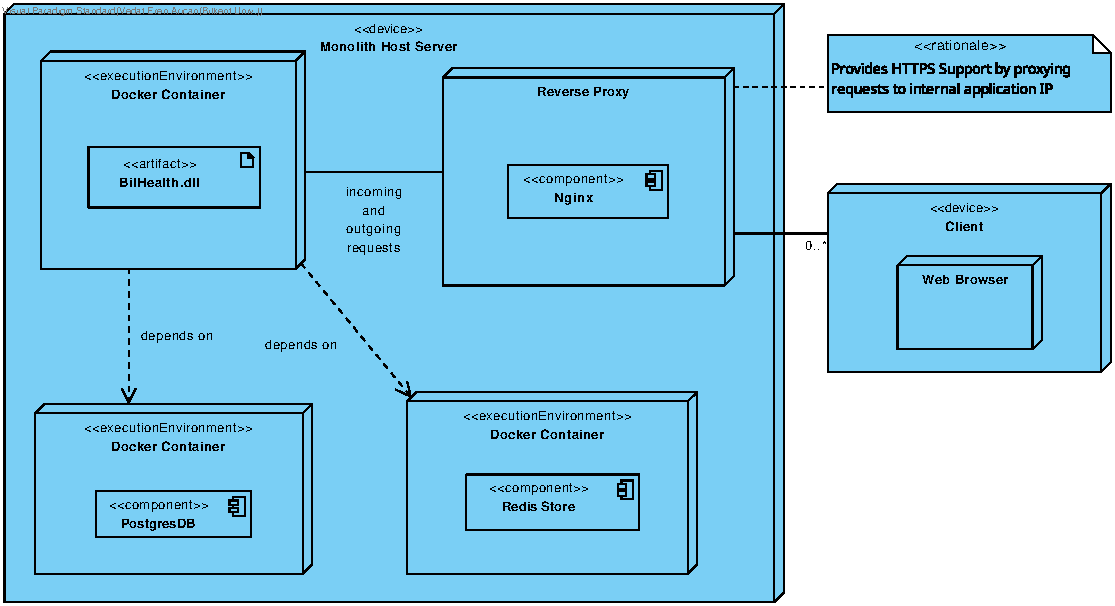
\includegraphics[width=\linewidth]{deploy_diag.pdf}

  \subsubsection{Termination}

  The application is terminated through the \texttt{docker-compose} tool.
  There are no special steps to be taken beyond commanding Docker to bring down the application containers.

  \subsubsection{Failure}

  The application does not crash in the event of failure.
  The implementation is careful to catch exceptions in appropiate places, and log the incidents if need be.
  Furthermore, the ASP.NET Core framework catches and reports any rare exceptions that may go unnoticed.

  Also, database access should be conducted through \textit{transactions}, which allow multiple operations to
  be made dependent on each other such that if one operation fails, the rest are not executed.
  This is ideal for data reliability and integrity in the event of failure.

  \pagebreak
  \section{Low-Level Design}

  \subsection{Object Design Trade-Offs}

  \begin{itemize}
    \item \textbf{Maintainability} versus \textbf{Performance:}
      The system will have objects for almost every part of the project because it is coded using OOP.
      This may cause a decrease in performance, but it is good for maintainability
      as it provides developers the mechanism to make changes easily.
    \item \textbf{Memory} versus \textbf{Performance:}
      The system will be created using OOP, so there will be many objects and classes involved
      during the execution of a given action on the application.
      This may cause some diminish in performance as memory is used by more objects and a bottleneck occurs.
    \item \textbf{Security} versus \textbf{Accessibility:}
      The system will not have security measures beyond a typical username and password.
      This decreases the security of the authentication process, but is better for accessibility purposes
      as users will not require extraordinary steps to access the system.
    \item \textbf{Functionality} versus \textbf{Extensibility:}
      As the system gains more functionality, despite the use of appropiate design patterns and practices,
      interfaces may become more rigid. This may cause the application to be less extensible.
  \end{itemize}

  \subsection{Final Object Design}

  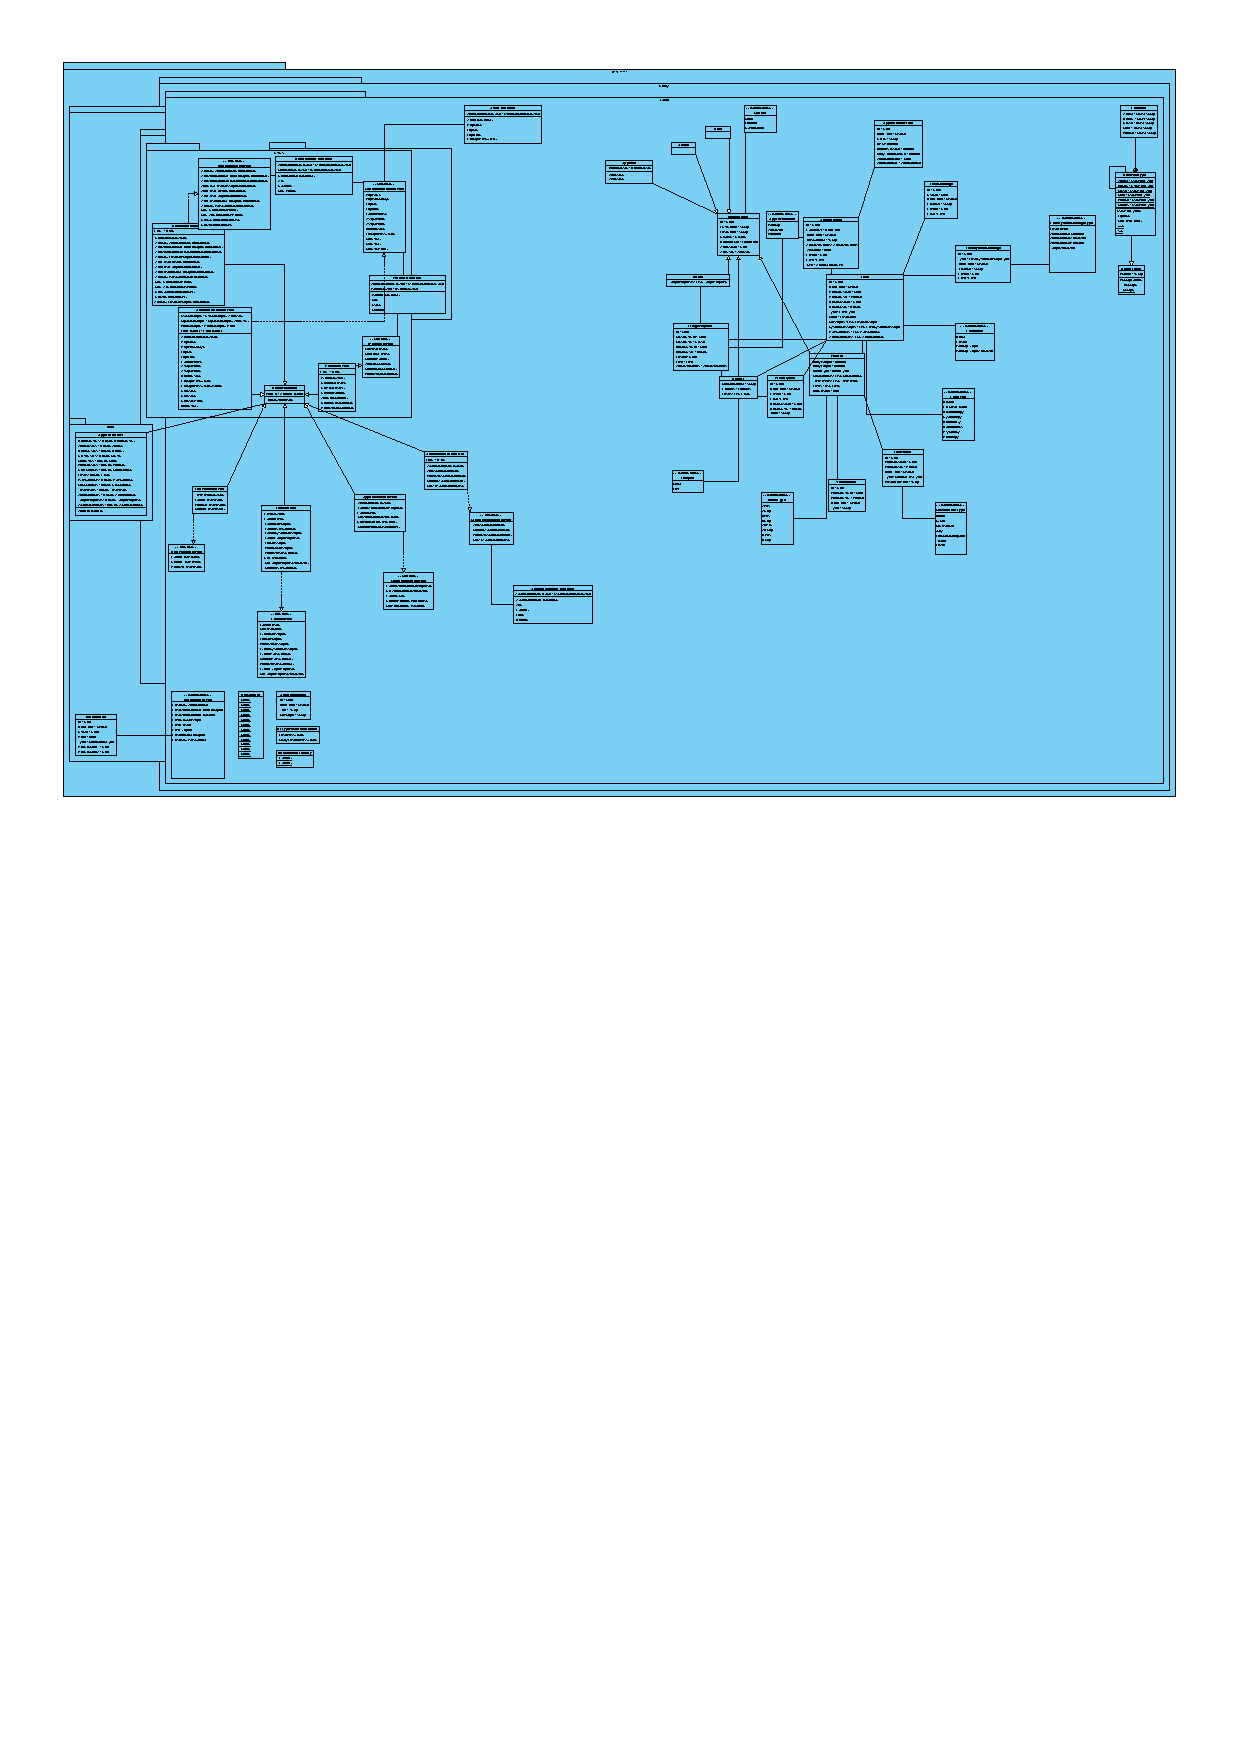
\includegraphics[width=\linewidth]{finalobject}

  \subsection{Packages}

  Below is a list of our namespaces with brief descriptions.
  Note that, to preserve the anonimity of the report, we've replaced the root namespace with a placeholder ``\texttt{Project}''.

  \begin{itemize}
    \item \texttt{Project.Utility}\textbf{:}\\
      This namespace contains the utility functions which were able to be decoupled from the project at large.
      In doing so, it can be used reliably across other namespaces.
    \item \texttt{Project.Utility.Enum}\textbf{:}\\
      This namespace contains the \textit{enum} and \textit{enum class} definitions that are used in many parts of the project.
    \item \texttt{Project.Services}\textbf{:}\\
      This namespace contains the main business logic interface through which boundary and entity systems are connected.
    \item \texttt{Project.Services.Users}\textbf{:}\\
      This namespace carries the same responsibility as its parent, but specifically for user-related entities.
    \item \texttt{Project.Model}\textbf{:}\\
      This namespace contains the entities that are persisted into a database. The main units of data are located here.
    \item \texttt{Project.Model.Identity}\textbf{:}\\
      This namespace contains entities that are specifically user information holding objects.
    \item \texttt{Project.Model.Dto}\textbf{:}\\
      This namespace contains \textit{record} objects that are used to transfer data to and from the front-facing controllers.
      It is also used for some internal communication of unpersisted data.
      In other words, these are temporary representations of the actual data entities to be persisted.
    \item \texttt{Project.Data}\textbf{:}\\
      This namespace contains the database context built from EF Core's repository-like architecture.
    \item \texttt{Project.Controllers}\textbf{:}\\
      This namespace contains the front-facing API endpoints through which external communication with clients take place.
  \end{itemize}

  \subsubsection{External Packages}

  \begin{itemize}
    \item \texttt{Microsoft.AspNetCore}\textbf{:}\\
      This package is the framework supporting the entire web application.
    \item \texttt{Microsoft.EntityFrameworkCore.Design}\textbf{:}\\
      This package allows the EF Core migration tool to work on the project.
    \item \texttt{Microsoft.AspNetCore.Diagnostics.EntityFrameworkCore}\textbf{:}\\
      This package allows debugging EF Core migrations.
    \item \texttt{npgsql.EntityFrameworkCore.PostgreSQL}\textbf{:}\\
      This package is the database driver providing EF Core its interoperation with PostgreSQL.
    \item \texttt{Microsoft.AspNetCore.Identity.EntityFrameworkCore}\textbf{:}\\
      This package provides authentication and authorization of users through integration with EF Core.
    \item \texttt{BCrypt.Net-Next}\textbf{:}\\
      This package provides the \textit{bcrypt} algorithm which is currently among the best in securely hashing user passwords.
    \item \texttt{Microsoft.AspNetCore.Mvc.NewtonsoftJson}\textbf{:}\\
      This package is the most popular JSON library for .NET, used as the default solution in most cases.
    \item \texttt{Microsoft.AspNetCore.SpaProxy}\textbf{:}\\
      This package allows the .NET build process to launch and proxy with the client application.
  \end{itemize}

  \subsection{Class Diagrams of Layers}

  \subsubsection{Data Access Layer}

  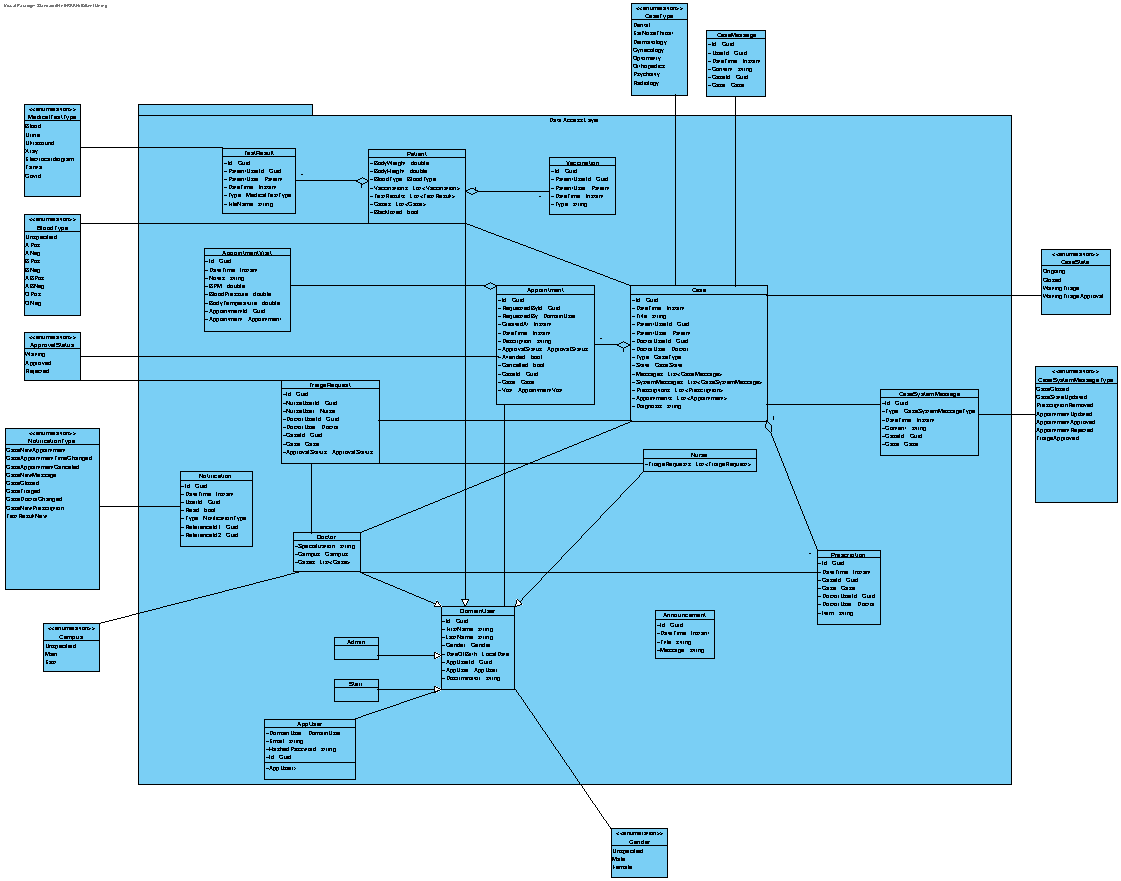
\includegraphics[width=\linewidth]{dataaccess}

  \subsubsection{Business Logic Layer}

  The diagrams on the two following pages are of the service and controller layers respectively.

  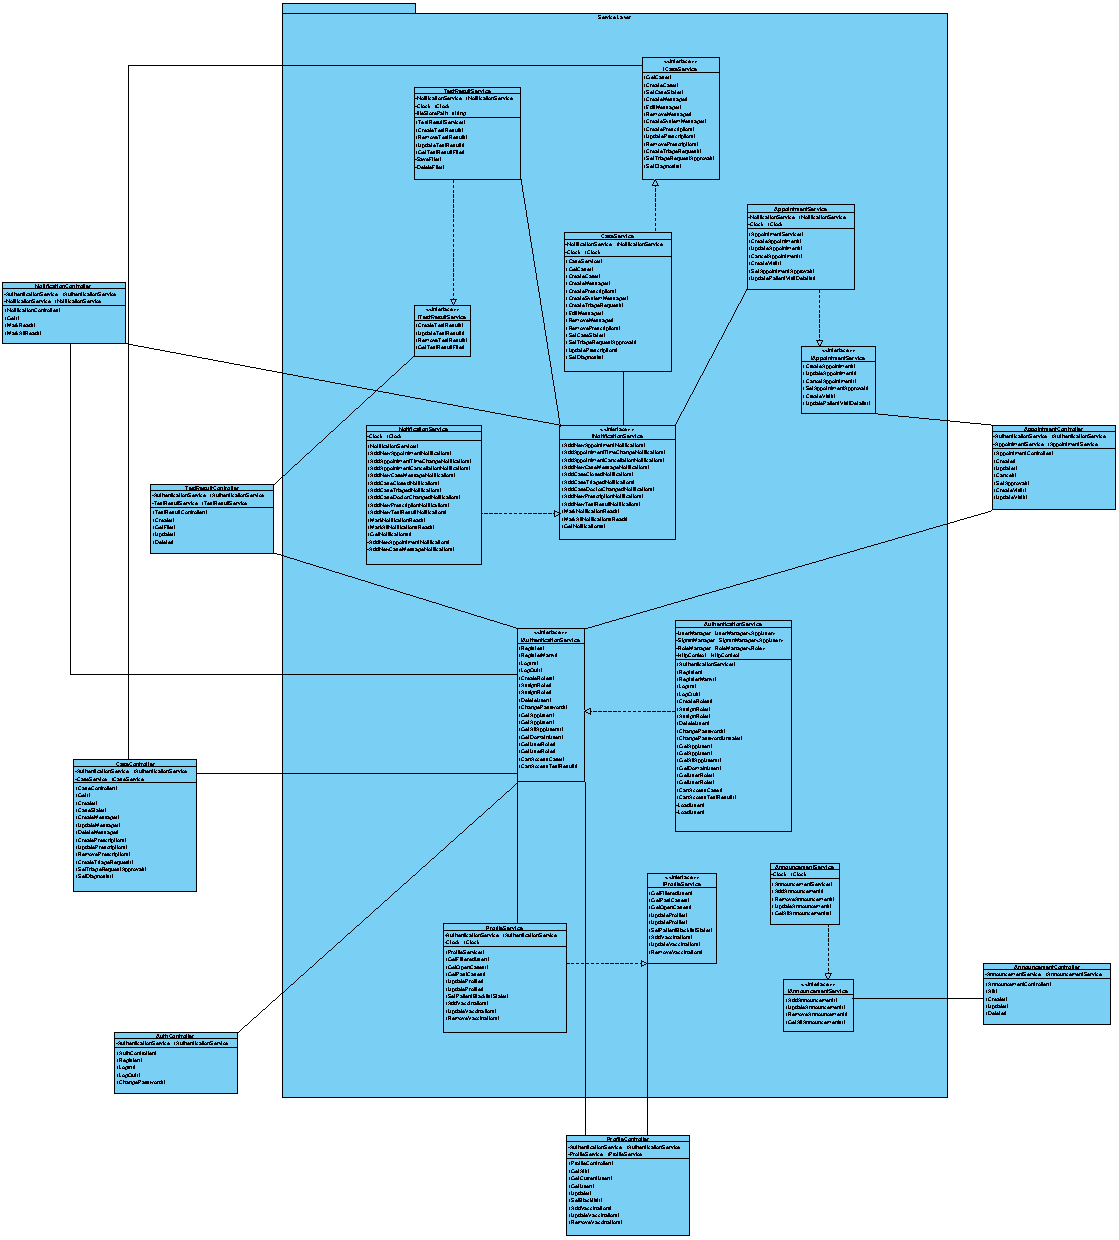
\includegraphics[width=\linewidth]{businesslogic}

  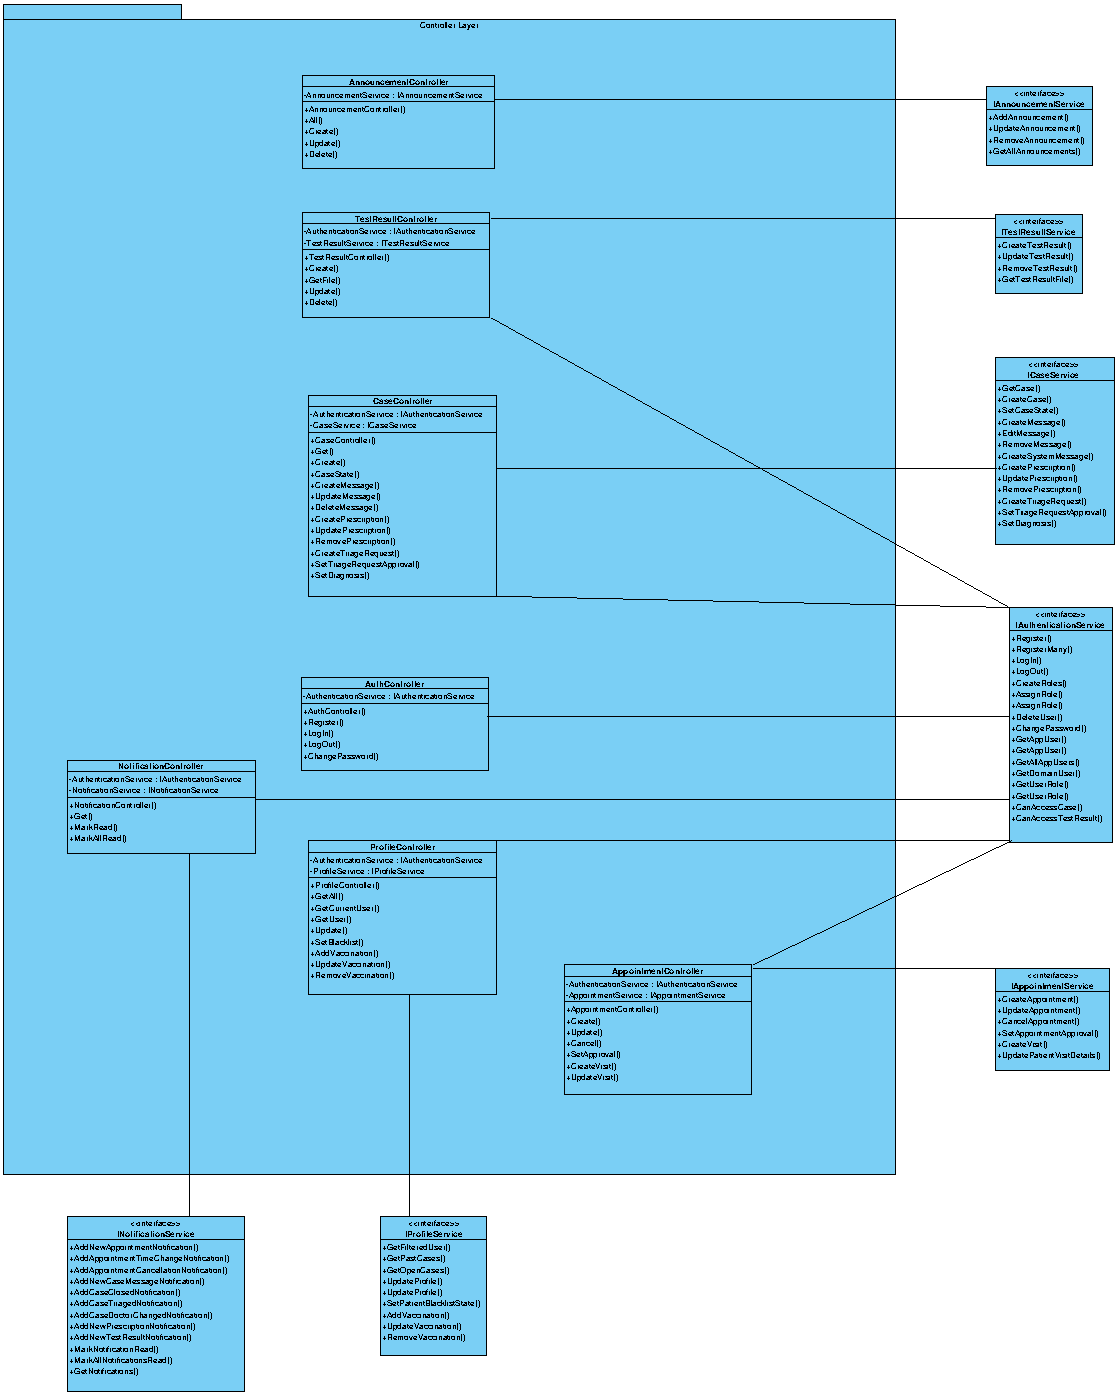
\includegraphics[width=\linewidth]{controller_layer}

  \pagebreak
  \subsubsection{User Interface Layer}

  Since the project uses React as its front-end technology, it is not possible to represent it in OOP fashion.
  However, we have drawn a diagram using the component names and relations.

  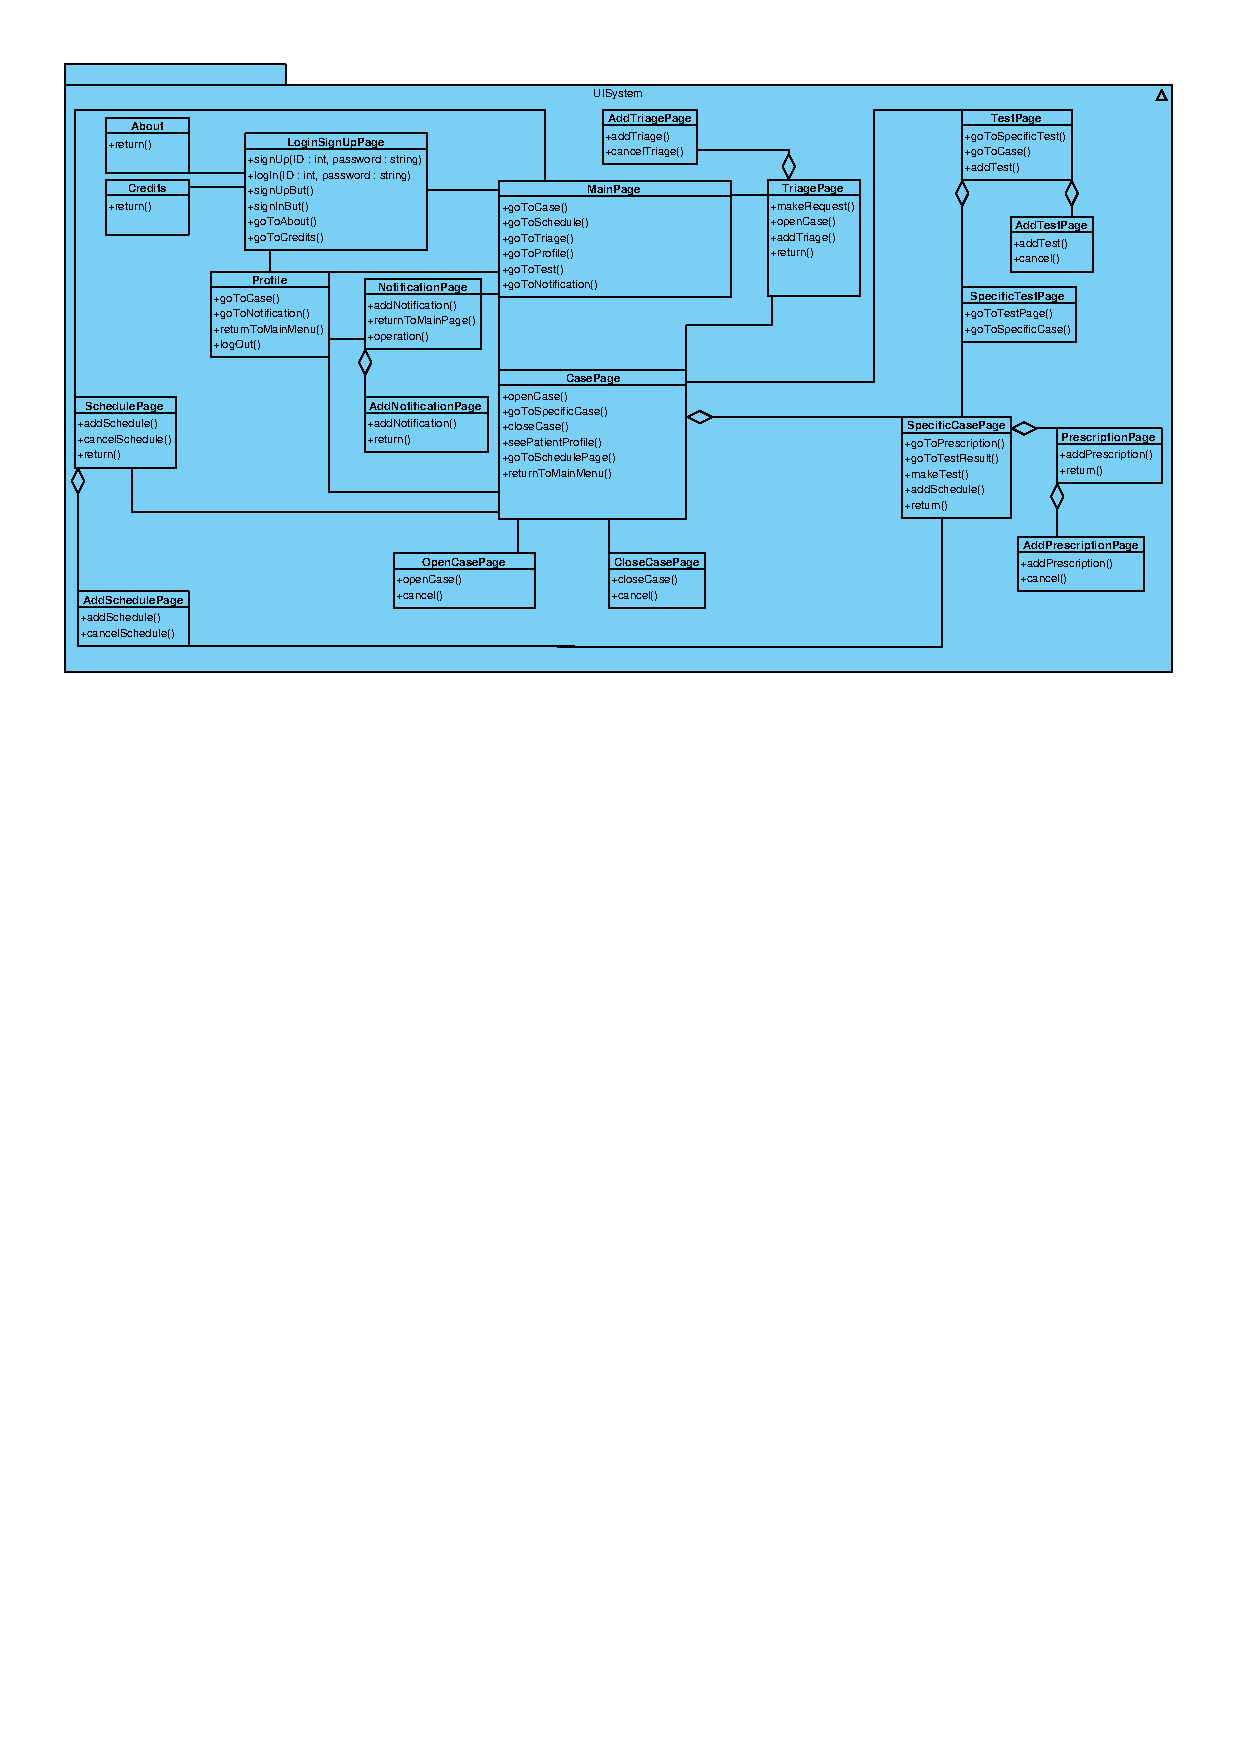
\includegraphics[width=\linewidth]{uisystem}

  \pagebreak
  \section{Glossary}

  \begin{itemize}
    \item \textbf{EF Core:} Microsoft's object relational mapper solution.
    \item \textbf{ORM:} Abbreviation for \textbf{O}bject \textbf{R}elational \textbf{M}apper.
    \item \textbf{.NET:} Microsoft's giant framework for C\# applications.
    \item \textbf{ASP.NET:} Microsoft's giant framework for web-based C\# applications.
    \item \textbf{PostgreSQL:} A popular relational database management system.
    \item \textbf{JSON:} Abbreviation for \textbf{J}ava\textbf{S}cript \textbf{O}bject \textbf{N}otation.
    \item \textbf{Hashing Passwords:} Cryptographically obscuring passwords such that they are practically irrecoverable.
    \item \textbf{Repository:} A very popular design pattern to provide an abstraction to persistent data.
    \item \textbf{API Endpoint:} The application programming interface endpoint through which communication with the system can occur.
    \item \textbf{Application Entrypoint:} The sum of the build process and configuration of the initialization of the system.
    \item \textbf{HTTP:} The most commonly used protocol over which web servers and clients communicate.
    \item \textbf{HTTPS:} Wraps the HTTP protocol into a cryptographically secured transmission protocol.
    \item \textbf{Enum:} A special type of programming entity that can be used to enumerate hard-coded types, mostly mapped to integers.
    \item \textbf{Enum Class:} An enum-like class adding specialized capability to the enum concept.
    \item \textbf{Record:} A C\# reference type with value-based equality.
    \item \textbf{Docker:} A software virtualization product.
    \item \textbf{Dependency Injection:} A software design pattern that inverses the dependency control by injecting dependencies into a dependent object.
  \end{itemize}

\end{document}
